To determine the distance to the supernova, we need to know a 
few important things for each day/data point of observation:
\\
We need:
\\
\\
$v$: The velocity of the expanding gas, Units: km/s.
\\
$t$: The time since explosion, Units: Julian Date.
\\
$t_0$: The time of explosion, Units: Julian Date.
\\
$z$: The time dialation factor, Unitless.
\\
$\theta$: The angular radius, Units: Degrees.
\\
\\
As seen in the figure \ref{fig:distance_graph}, we have 5 data points. 
For each of these data points, we have a $t$, $v$, and $\theta$.
\\
\\
First we start with velocity $v$. This is determined by looking at 
the spectrum of the expanding photosphere and seeing how much it is blueshifted compared to 
a source nearby. This will tell us how fast the expanding gas is moving towards us, thus 
giving us a velocity.
\\
\\
Next we will find the time $t$, which is as easy as using a device that tells you the 
julian date\footnote{Julian date is the number of days (and fractions of days) 
since 12:00 PM November 24, 4714 BC.} of the time of observation. 
\\
\\
$t_0$ is a bit harder to find because we dont always see exactly when a supernova 
happens, often we find out a few dats after the fact. So for this analysis we used two methods.
\\
Method 1: 
\\
We calculate the line of best fit normally, which tells us the distance $d$ and the time of explosion $t_0$.
\\
Method 2: 
We calculate the line of best fit but set the y-intercept, $t_0$, to zero, and calculated the distance.
\\
\\
The time dialation factor $z$ is calculated using spectroscopy, looking at spectrums of the light and determing 
how much time will be dialated from traveling from the direction of the supernova. This is something that needs 
to be looked up. We did not calculate this ourselves.
\\
\\
\\
\\
\\
\\
\\
\\
\\
\\
\\
\\
\\
\\
\\
\\
\\
\\
\\
\\
Now, we have the angular radius $\theta$. Determinig the angular radius is the most difficult part of this project,
and requires a large amount of data. To start off, we will look at the equation for calculating $\theta$, which is derived in
this paper by Mitchell \cite{mitchell_locating_2023}.
\begin{equation}
    \log{\theta} = -\log{\zeta_{\lambda^{\textrm{'}}}}-0.2(m_\lambda-A_\lambda-b_{\lambda^{\textrm{'}}})+0.5\log{(1+z)}
\end{equation}
Or with $\theta$ isolated,
\begin{equation}
    \theta = 10^{-\log{\zeta_{\lambda^{\textrm{'}}}}-0.2(m_\lambda-A_\lambda-b_{\lambda^{\textrm{'}}})+0.5\log{(1+z)}}
\end{equation}
\\
\\
To break this equation down, here are the component parts:
\\
$m_\lambda$: The magnitude of the filter used. We will be using the B and V filter 
separately, so we will have two different distances.
\\
\\
$A_\lambda$: The extinction factor. This value accounts for any interference from gas in the space between the observed
object and the observer. This includes the athmosphere.
\\
\\
$z$: The time dialation factor. This is explained more above.
\\
\\
$\zeta_{\lambda^{\textrm{'}}}$: This is the dilution factor. This helps us get more accurate numbers and 
accounts for any sort of distortion effects. It is a temperature-dependant polynmial with the form of this 
\ref{eqn:zeta} equation below and with constants $a_i$ pulled from the paper by Hamuy \cite{hamuy_distance_2001}
and are specific for the filter used for observation, in our case we used the B and V filter so we will be using the B-V values.
\begin{equation}\label{eqn:zeta}
    \zeta_{\lambda^{\textrm{'}}}(T) = \sum_{i=0}^{2}a_i(\frac{10^4K}{T})^i
    ,a_i = (0.7557, -0.8997, 0.5199)
\end{equation}
\\
\\
$b_{\lambda^{\textrm{'}}}$: This is the synthetic magnitude at the wavelength $\lambda$. It is also a 
temperature-dependant polynmial with the form below. The values for $c_{i,\lambda}$ were also pulled from the paper
by Hamuy \cite{hamuy_distance_2001}, which were modified from Estmans \cite{eastman_atmospheres_1996} calculations.
The values for $c_{i,\lambda}$ depend on the filter (wavelength of light) used for the calculation and will depend on
which way you measure temperature, which will be mentioned below.
\begin{equation}\label{eqn:synth_mag}
    b_{\lambda^{\textrm{'}}}(T) = \sum_{i=0}^{5}c_{i,\lambda}(\frac{10^4K}{T})^i
\end{equation}
\\
\\
\\
\\
\\
The last thing needed is to determine the temperature of the expanding gas at a certain time. Though there are many different methods
that can be used, we will be using the one called Color Temperature. This method is defined in the paper by Matthews and Sandage \cite{matthews_optical_1963}.
\\
\\
We use two filters, in our case the B and V filters. We find the B-V values and their corresponding temperature values listed in the 
Matthews and Sandage \cite{matthews_optical_1963} paper. We use the equation below to calculate the line of best fit, which gives 
our K and C values (slope and intercept of line of best fit).
\begin{equation}\label{eqn:kandc}
    \frac{10000k}{T} = K(B-V)+C
\end{equation}
When finding the line of best fit of this equation \ref{fig:bv_temp}, you get a K of 1.58 and a C of 0.72. 
It is suggested by Matthews and Sandage \cite{matthews_optical_1963}
that a C of 0.48 should be used for a Type-II supernova observation.
\begin{figure} [h!]
    \begin{center}
    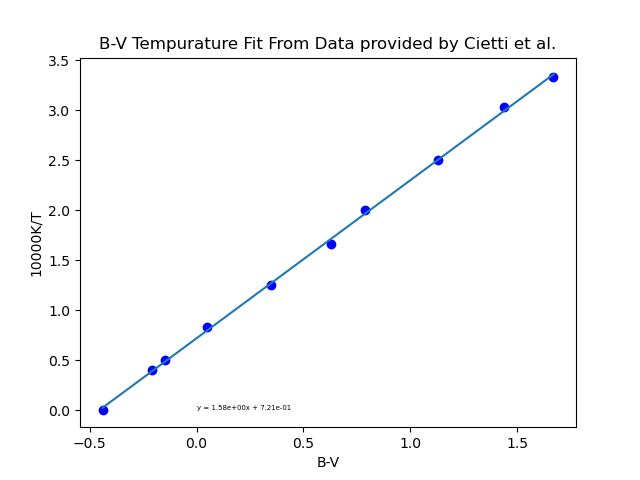
\includegraphics[width=0.5\textwidth]{B-V_Temperature_fit.png}
    \end{center}
    \label{fig:bv_temp}
    \caption{The temperature fit for B-V filters.}    
\end{figure}
\\
\\
When we rearrange equation \ref{eqn:kandc} to isolate temperature $T$, we get:
\begin{equation}
    T = \frac{10000}{K(B-V)+C}
\end{equation}
Now we correct for any errors in the B and V values:
\begin{equation}\label{eqn:temperature}
    T = \frac{10000}{K((B-B_\textrm{correction})-(V-V_\textrm{correction}))+C}
\end{equation}
When we plug in our values for B and V, the B and V correction factors, and the K 
and suggested C values into the temperature equation \ref{eqn:temperature} 
above, we get the temperature of the expanding gas during the observation time.
\\
\\
Now that we have all the data nessisary, we can calculate the distance.
